\clearpage
\subsection{Design}

\subsubsection{scope}
\par{The design module allows the designer/design team to structure the layout of the book.This is done by creating or choosing a template, as well as uploading all desired graphics and designing the books cover pages.}

\begin{figure}[h]
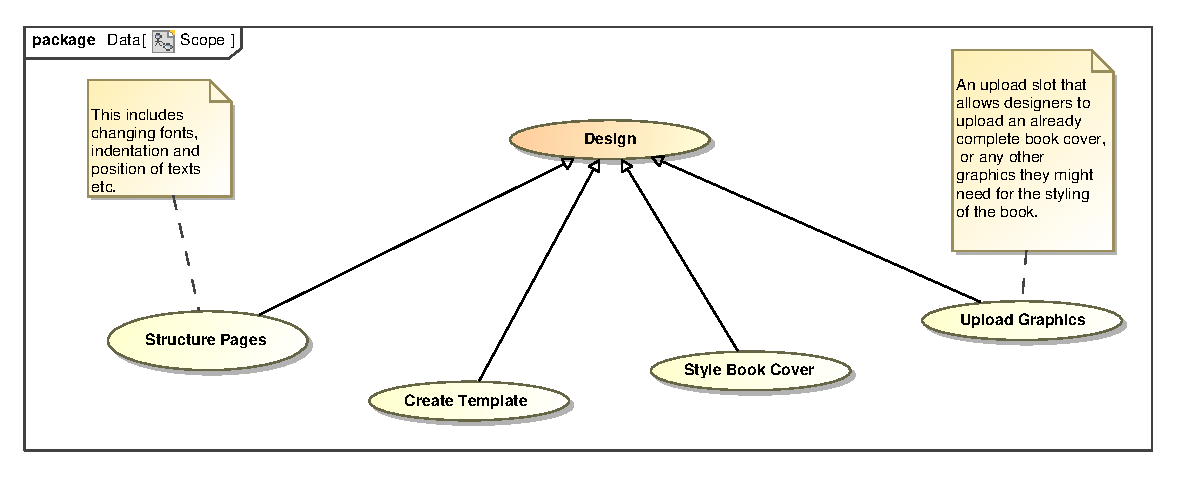
\includegraphics[scale=0.9,width=450px]{epsImages/Design/Scope.eps}
\centering
\caption{Scope of Design module}
\end{figure}

\newpage
\subsubsection{Use Cases}
\begin{enumerate}
\item \textbf{Structure Pages - priority: critical}
\par{This use case which allows one to structure the  manuscript.}
\par{\textbf{Service Contract:}
}
\begin{figure}[h]
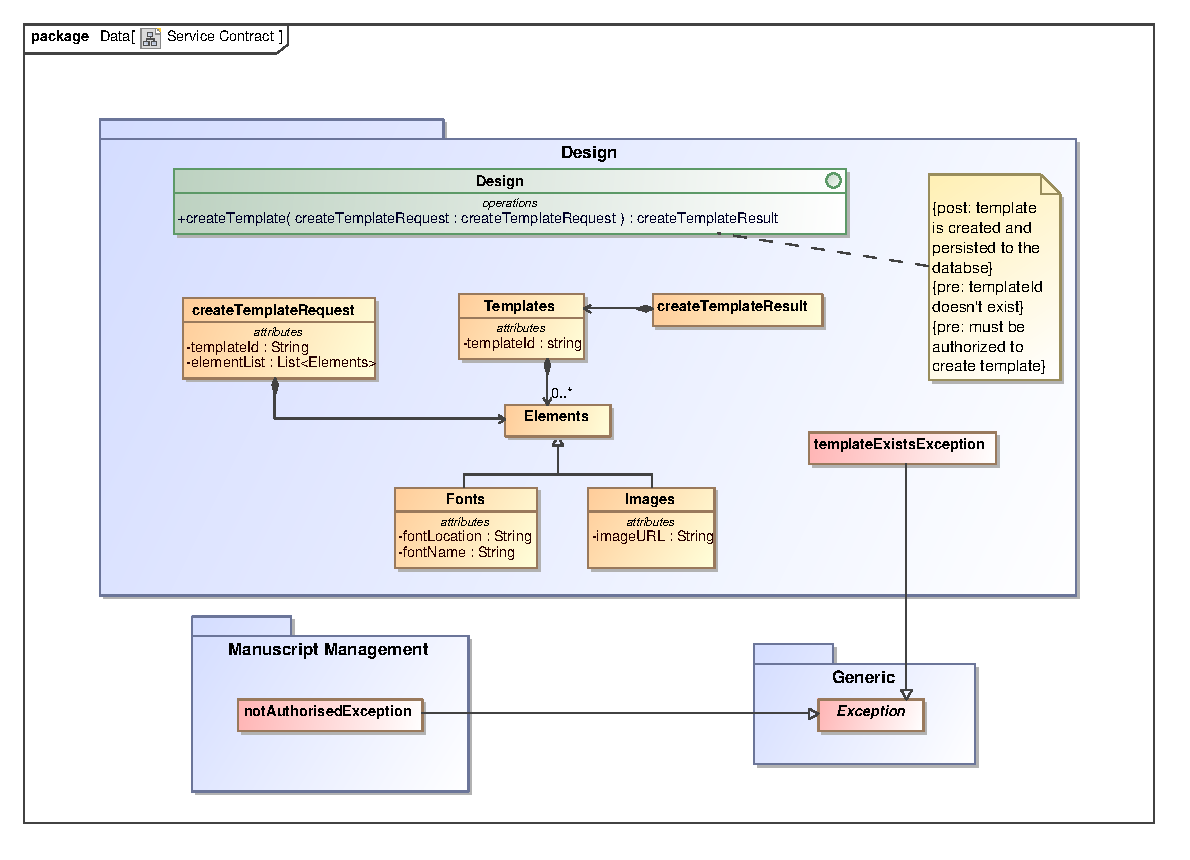
\includegraphics[scale=0.8,width=400px]{epsImages/Design/createTemplateServiceContract.eps}
\centering
\caption{Service contract for structuring a menuscript}
\end{figure}

\newpage
\item \textbf{Create Template - priority: nice to have}
\par{This module allows a user to create a template design for the book.}
\par{\textbf{Service Contract:} 
}
 \begin{figure}[h]
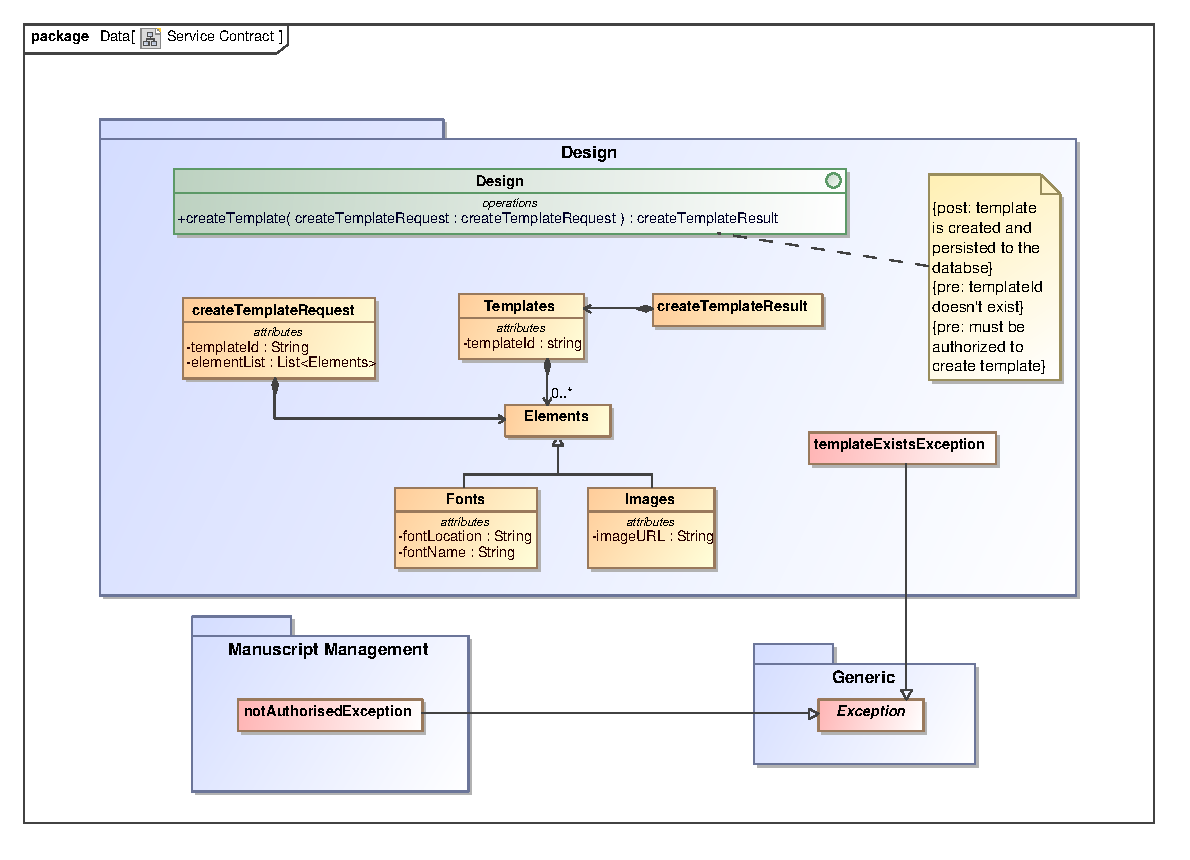
\includegraphics[scale=0.8,width=400px]{epsImages/Design/createTemplateServiceContract.eps}
\centering
\caption{Service contract for creating a template design}
\end{figure}

\newpage
\item \textbf{Create Book Cover - priority: critical}
\par{This use case which allows create a book cover for a  manuscript.}
\par{\textbf{Service Contract:} 
}
 \begin{figure}[h]
\centering
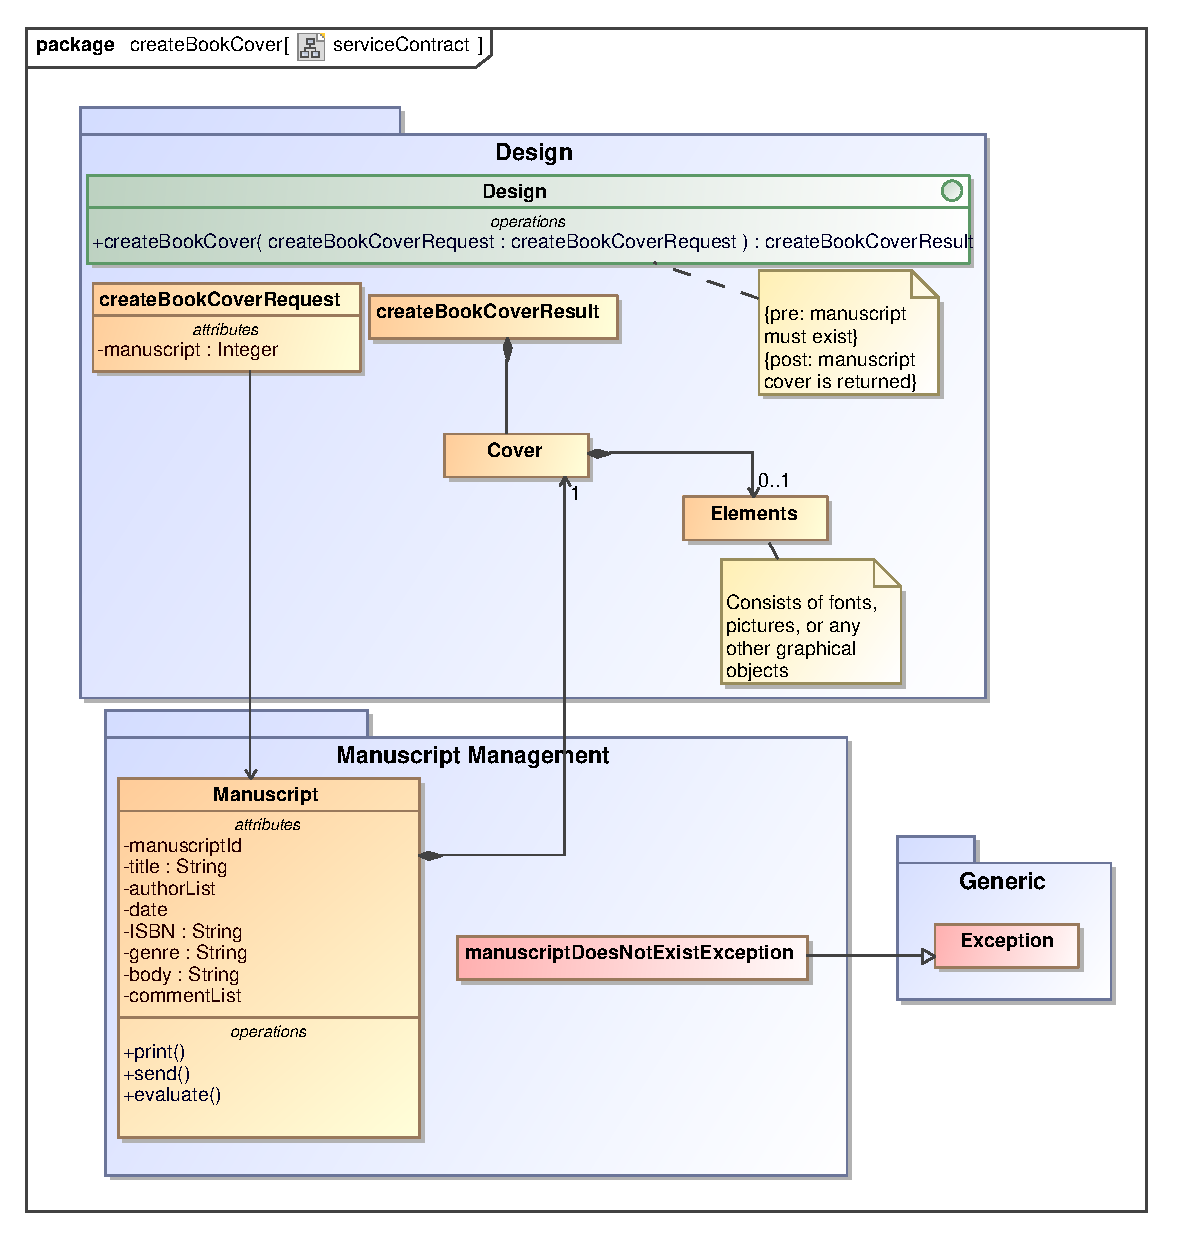
\includegraphics[scale=0.8,width=400px]{epsImages/Design/createBookCover.eps}
\caption{Service contract for creating a book cover}
\end{figure}

\newpage
\item \textbf{Upload Graphic - priority: important}\\
\par{This use case allows a user to open any graphic they choose. This may be a new font, or image they wish to use, or a completed cover for the book. Size and format of a graphic are restricted however.}
\par{\textbf{Service Contract:}}
\begin{figure}[h]
\centering
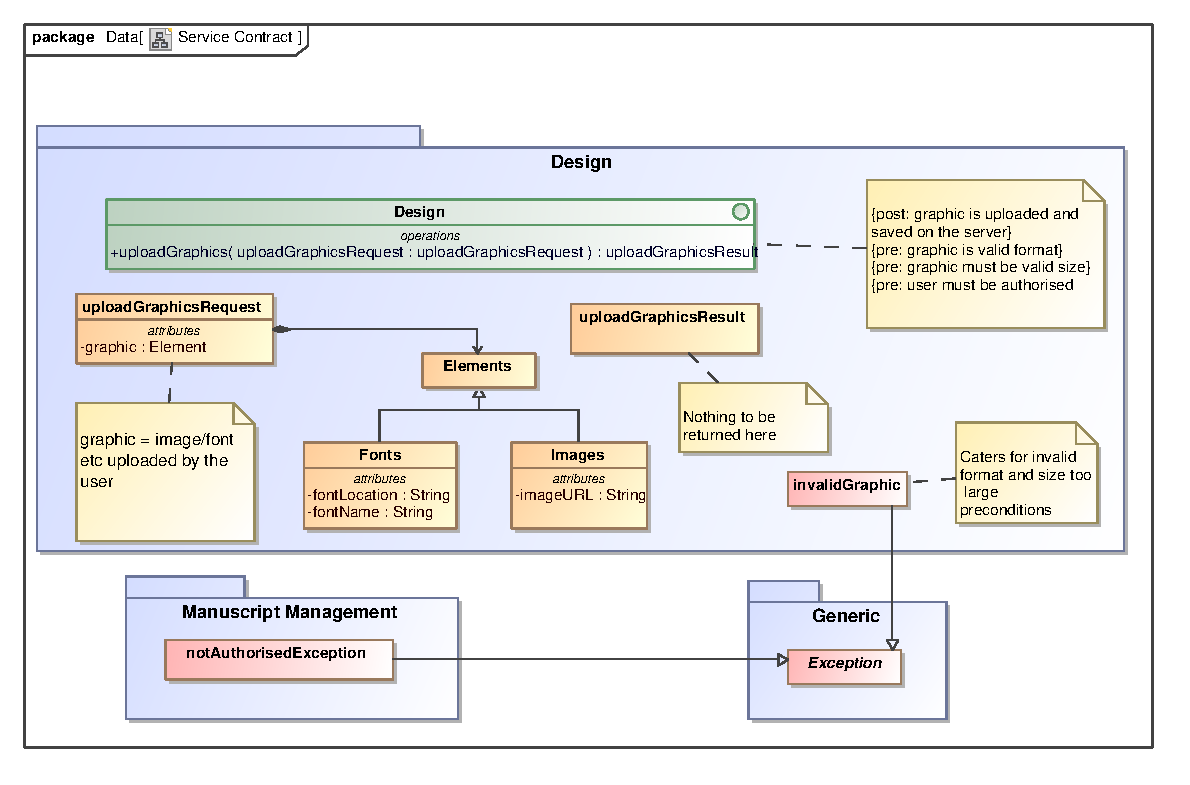
\includegraphics[scale=0.8,width=400px]{epsImages/Design/uploadGraphicsServiceContract.eps}
\caption{Service contract for uploading a graphic}
\end{figure}
\end{enumerate}

\newpage
\subsubsection{Domain Model}
\par{The design elements of the designers role is accommodated in this package. It works with elements of the Manuscript Management package as it manipulates the manuscript. }

\begin{figure}[h]
\centering
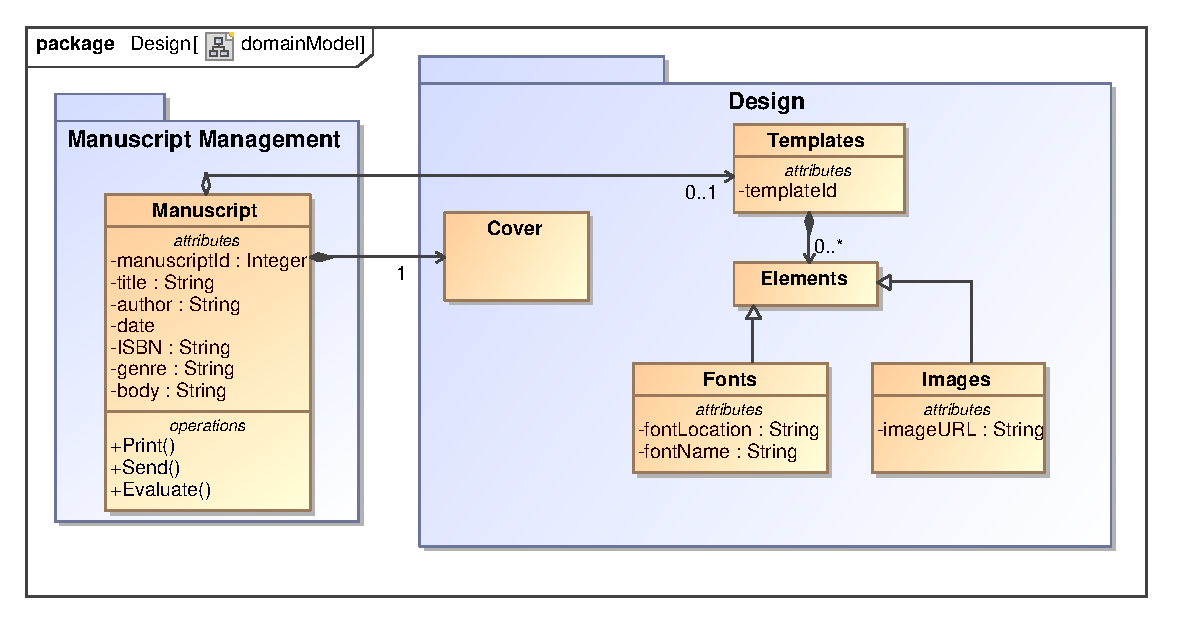
\includegraphics[scale=0.8,width=400px]{epsImages/DomainModels/DesignDomainModel.eps}
\caption{Design module's Domain Model}
\end{figure}
